% !TeX root = spherical_harmonics.tex
% !TeX spellcheck = de_DE
\subsection{Die Suche nach einer guten Basis}
Auch wenn wir eingangs in unserem Kurs so sehr über Basen geschimpft haben\footnote{Wir wollen keine Namen nennen, aber Johannes war besonders hartnäckig...}, so ist uns natürlich bewusst, dass gerade für effiziente Berechnungen eine Basis praktisch immer gewählt wird. Welche Basis man wählt, ist dabei von großer Bedeutung: Andrea hat in ihrer Doktor-Arbeit eine bestimmte Berechnung, welche z.B. zur Modellierung von Luftbewegung millionenfach wiederholt genutzt werden soll, um den Faktor 1000 verschnellern können, und das nur durch geschickte Basiswahl. 

\begin{remark}
	Meistens ist eine Basis geschickt gewählt, wenn sie orthogonal bzgl. eines zum Problem passenden Skalarprodukts ist. Nun gibt es aber viele Skalarprodukte, die man wählen kann, die durchaus auch unterschiedliches Verständnis von Orthogonalität festlegen.
\end{remark}
Schauen wir uns einmal einige Beispiele für mögliche Skalarprodukte auf dem Raum der Polynome an:
\begin{example}
	Sei $B$ die Kugel in $\IR^3$ mit Radius 1. Dann ist mit
	\begin{align*}
		\braket{f,g}_B :&= \int_B f g \dd B
	\end{align*}
	ein Skalarprodukt auf dem Raum der Polynome gegeben.
\end{example}

\begin{example}
	Sei $Z$ ein Zylinder in $\IR^3$, z.B. mit Radius und Höhe 1. Dann ist mit
	\begin{align*}
		\braket{f,g}_Z :&= \int_Z f g \dd Z
	\end{align*}
	ein Skalarprodukt auf dem Raum der Polynome gegeben.
\end{example}

\begin{example}
	Sei $K$ ein Kegelstumpf in $\IR^3$, z.B. mit oberen Radius und Höhe 1 sowie unterem Radius $\frac{1}{2}$. Dann ist mit
	\begin{align*}
		\braket{f,g}_K :&= \int_K f g \dd K
	\end{align*}
	ein Skalarprodukt auf dem Raum der Polynome gegeben.
\end{example}

\begin{example}
	Sei $Q$ ein Quader in $\IR^3$, z.B. mit den Kantenlängen 1, 2 und 3. Dann ist mit
	\begin{align*}
		\braket{f,g}_Q :&= \int_Q f g \dd Q
	\end{align*}
	ein Skalarprodukt auf dem Raum der Polynome gegeben.
\end{example}

\begin{centralquestion}
Wäre es nicht praktisch, eine Basis zu finden, die für möglichst viele Skalarprodukte orthogonal ist? Wie würdet ihr mit dem neu erworbenen Wissen nach solch einer Basis suchen?

Diskutiert über eure Ansätze und versucht einen Algorithmus zu entwickeln, der eine möglichst allgemein einsetzbare Basis konstruiert.
\end{centralquestion}

\pagebreak
%\begin{remark}
%Am besten wählt man eine Basis, die möglichst gut an das gegebene Problem angepasst ist, doch was genau heißt das? Für die Auswahl an Problemen in diesem Kurs haben wir festgelegt, dass es sich um Probleme in unserer physikalischen Welt handeln soll. Wir haben uns bereits angeschaut, wie sich diese Einschränkung mathematisch äußert: Alles was wir messen wollen, muss natürlich, also $O_3$-verträglich sein. Wir haben uns auch schon mit der Darstellungstheorie von $O_3$ und einigen ihrer Untergruppen beschäftigt und festgestellt, dass $O_3$ den Raum der Polynome (oder äquivalent: den Raum der symmetrischen Tensoren) in irreduzible Unterräume zerlegt.
%\end{remark}
%\begin{remark}
%Die irreduziblen Unterräume sind besonders: Wir haben bereits sehr gut verstanden, dass sie immer (also für jedes $O_3$-verträgliche Skalarprodukt) senkrecht zueinander stehen und dass lineare Abbildungen zwischen zwei irreduziblen Unterräumen entweder 0 oder ein Vielfaches der Identität sein können. Wenn man also eine lineare Wirkung berechnen möchte, erspart man sich durch die Zerlegung in irreduzible Unterräume einiges an Arbeit: Alles, was zu bestimmen ist, sind die Konstanten, mit der die Identität zwischen zwei zueinander isomorphen irreduziblen Unterräumen koppeln.
%\end{remark}
%\begin{remark}
%Im übrigen: Für bilineare Abbildungen ist es etwas komplizierter, aber die grundsätzliche Aussage bleibt bestehen: Alle Abbildungen sind entweder 0 oder Vielfache einer Identität (auch dann wenn die Identität etwas komplizierter zu berechnen ist).
%\end{remark}
%\begin{remark}
% All dies legt nahe, dass eine Basiswahl, die an die irreduziblen Unterräume angepasst ist, praktisch immer eine gute Idee ist. Jetzt sind diese irreduziblen Unterräume aber allermeistens nicht ein-dimensional, wie sucht man sich nun eine möglichst kanonische Basis aus?
%\end{remark}
%\begin{remark}
%	\label{rem:einbettung_in_physik}
% Hinzu kommt, dass die irreduziblen Unterräume zwar für ganz $O_3$ irreduzibel sind, aber es gibt einige Probleme in der Physik, die eher einer Einbettung von $O_2$ in $O_3$ gleichen, z.B. (Teilchen-) Kollision an einer Wand, eine ausgezeichnete Richtung haben, z.B. die Bewegung von geladenen Teilchen durch einen Kondensator, oder rotierende Systeme beschreiben (Einbettung von $SO_2$ in $O_3$.
%\end{remark}
%
% \begin{remark}
% 	Idealerweise ist unsere Basis auch für solche Fälle ausgelegt. Es stellt sich heraus, dass beide Probleme gleichzeitig gelöst werden können.
% \end{remark}

% \begin{remark}
% 	Idealerweise ist unsere Basis auch für solche Fälle ausgelegt. Es stellt sich heraus, dass beide Probleme gleichzeitig gelöst werden können.
 %\end{remark}
 \subsection{Die Gelfand-Zetlin Basis}
 \begin{definition}[Konstruktion der $\Gae\jae\el\soft\fae\aaa\en\dae$-$\Zae\jae\tae\el\iii\en$-$\Bae\aaa\sae\iue$ (Gelfand\footnote{Israel Gelfand, $\I\sae\rae\aaa\iii\el\soft$ $\Em\ooo\iii\ssae\jae\jae\wae\iii\tschae$ $\Gae\jae\el\soft\fae\aaa\en\dae$ (1913--2009), sowjetischer Mathematiker}-Zetlin\footnote{Michael Zetlin, $\Em\iii\xa\aaa\iii\el$ $\El\soft\wae\ooo\wae\iii\tschae$ $\Zae\jae\tae\el\iii\en$ (1924--1966), russ. Mathematiker und Physiker; Der Name wird leider auf viele verschiedene Weisen transkribiert, u.A. eben Zetlin (meist im dt. Sprachraum), aber auch Tsetlin (engl. Sprachraum), Cetlin, Tzetlin, Zeitlin, Zetlin}-Basis]
 	\label{def:konstruktion_gz_basis}
	Sei $G$ eine Gruppe mit halb-einfacher Darstellung auf einem Vektorraum $V$ und $U^i_0$ einer der irreduziblen Unterräume von $V$. Für diesen Unterraum wird eine \emph{Gelfand-Zetlin-Basis} wie folgt konstruiert:
	\begin{enumerate}[label={\arabic*.)}]
		\item Setze das Level $k=0, H_0 = G$
		\item Bestimme für jeden Unterraum $U_k^i$: \label{def:gz_it_anfang}
		\begin{enumerate}
			\item Berechne $\dim{U_k^i}$
			\item Ist $U_k^i$ 1-dimensional? Dann wähle einen von Null verschiedenen Vektor aus $U_k^i$ als einen der Basisvektoren von $U^1_0$.
			\item Ist $U_k^i$ mehr als $1$-dimensional? Dann merke dir $U_k^i$ für den nächsten Schritt.
		\end{enumerate}
		\item Wähle geschickt eine Untergruppe $H_{k+1}$ von $H_k$, sodass jeder Unterraum $U_k^i$ mit $\dim{U_k^i}>1$ in paarweise nicht-isomorphe für $H_{k+1}$ irreduzible Unterräume  zerfällt. (Klappt dies nicht, ist entweder eine andere Untergruppe zu finden, oder es gibt keine Gelfand-Zetlin-Basis). \label{def:gz_it_ugschritt}
		\item Nummeriere die Unterräume des nächst-höheren Levels: Nenne alle für $H_{k+1}$ irreduziblen Unterräume $U_{k+1}^{1}, U_{k+1}^{2}, \ldots$, inklusive der bereits für $H_k$ 1-dimensionalen Unterräume.
		\item Erhöhe das Level um 1: $k++$. \label{def:gz_it_ende}
		\item Wiederhole die Schritte \ref{def:gz_it_anfang} bis \ref{def:gz_it_ende}, bis alle Unterräume vom nächst-höheren Level 1-dimensional sind.
		\item $k_{\text{max}} = k$
		\end{enumerate}
\end{definition}
\begin{remark}
	Formal betrachtet, brauchen die 1-dimensionalen Untervektorräume nicht für Schritt \ref{def:gz_it_ugschritt} ausgeschlossen werden. Sie werden für jede Untergruppe 1-dimensional bleiben und sich nicht weiter ändern, entsprechend braucht man sie für die weiteren Schritte auch nicht zu berücksichtigen.
\end{remark}
\begin{definition}[$\Gae\jae\el\soft\fae\aaa\en\dae$-$\Zae\jae\tae\el\iii\en$-$\Dae\jae\rae\jae\wae\ooo$ (Gelfand-Zetlin-Baum)]
	Mit der Konstruktion nach \ref{def:konstruktion_gz_basis} bauen wir einen Baum mit $k_{\text{max}}+1$ Leveln. Der Stammknoten ist $U_0^i$, die Blätter sind alle gefundenen 1-dimensionale Unterräume. Die Knoten zwischen dem Stammknoten und den Blättern entsprechen den irreduziblen Unterräumen der jeweiligen Level, die Kanten verbinden einen irreduziblen Unterraum $U$ eines Levels mit allen irreduziblen Unterräumen des nächst-höheren Levels, die aus $U$ im Schritt \ref{def:gz_it_ugschritt} herauskommen. Eindimensionale Unterräume, die bereits in kleineren Leveln auftreten, werden hier als Knoten auf jedem höheren Level wiederholt bis zum maximalen Level.
	Diesen Baum nennen wir \emph{Gelfand-Zetlin-Baum}. Er kann z.B. wie folgt aussehen:
	\begin{align*}
		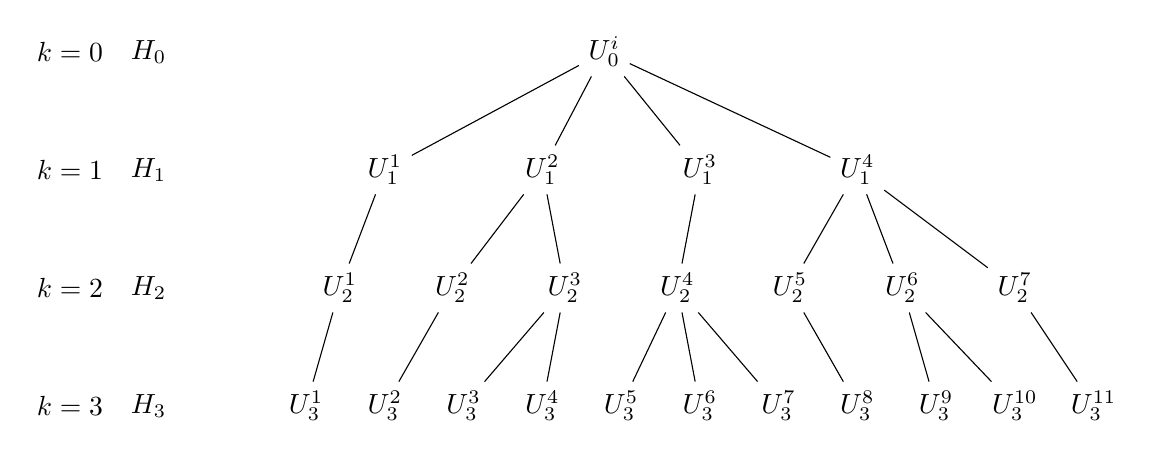
\begin{tikzpicture}[baseline={([yshift=-2ex]current bounding box.center)}]
			\foreach\x  in {1,2,...,11}{
				\node (u3\x) at (\x,-4.5){$U_3^{\x}$};
			}
%			\foreach\x  in {1,2,3.5,6,8,9.5,11}{
%				\node (u2\x) at (\x,-3){$U_2^{\x}$};
%			}
			\foreach\x [evaluate=\x as \y using {\x*10/7}] in {1,2,...,7}{
				\node (u2\x) at (\y,-3){$U_2^{\x}$};
			}
%			\foreach\x  in {1,2.75,6,9.5}{
%				\node (u1\x) at (\x,-1.5){$U_1^{\x}$};
%			}
			\foreach\x [evaluate=\x as \y using {\x*10/5}] in {1,2,...,4}{
				\node (u1\x) at (\y,-1.5){$U_1^{\x}$};
			}
			\node (u0) at (4.7875,0){$U_0^i$};
			\foreach\x in {1,2,...,4}{
				\draw[] (u0) to (u1\x);
			}
			\draw[] (u11) to (u21);
			\draw[] (u12) to (u22);
			\draw[] (u12) to (u23);
			\draw[] (u13) to (u24);
			\draw[] (u14) to (u25);
			\draw[] (u14) to (u26);
			\draw[] (u14) to (u27);
			\draw[] (u21) to (u31);
			\draw[] (u22) to (u32);
			\draw[] (u23) to (u33);
			\draw[] (u23) to (u34);
			\draw[] (u24) to (u35);
			\draw[] (u24) to (u36);
			\draw[] (u24) to (u37);
			\draw[] (u25) to (u38);
			\draw[] (u26) to (u39);
			\draw[] (u26) to (u310);
			\draw[] (u27) to (u311);
			\foreach\x [evaluate=\x as \y using {-\x*1.5}] in {0,1,...,3}{
				\node (l\x) at (-2,\y){$k=\x$};
				\node (h\x) at (-1,\y){$H_{\x}$};
			}
		\end{tikzpicture}
	\end{align*}
	In einem Gelfand-Zetlin-Baum sind alle Darstellungen paarweise ungleich. Es kann aber auftreten, dass manche Darstellungen isomorph zueinander sind (wobei die Kinder eines Knotens niemals isomorph zueinander sein dürfen).
\end{definition}
\begin{remark}
		Die Wahl der Untergruppen-Kette $H_1,\ldots,H_{k_{\text{max}}}$ ist hier spielentscheidend und keinesfalls eindeutig. Aus diesem Grund gehört zu einer vollständigen Anweisung \enquote{Wähle eine Gelfand-Zetlin-Basis für $G$ auf $V$} auch die Angabe der Untergruppenkette $H_1,\ldots,H_{k_{\text{max}}}$.
\end{remark}
\begin{remark}
	Auch wenn die Konstruktion einer Gelfand-Zetlin-Basis klappt, hat man nicht unbedingt etwas gewonnen. Wenn man dazu besonders exotische Untergruppen benutzen muss, bringt einem die Gelfand-Zetlin-Basis in der Anwendung nicht besonders viel. Eigentlich möchte man sich erst für eine Untergruppenkette $H_0,\ldots,H_{k_{\text{max}}}$ entscheiden und dann schauen, ob die Konstruktion funktioniert.
\end{remark}
\begin{definition}[$\Gae\jae\el\soft\fae\aaa\en\dae$-$\Zae\jae\tae\el\iii\en$-$\Bae\aaa\sae\aaa$]
	\label{def:gz_basis}
	Sei $G$ eine Gruppe mit Darstellung auf einem Vektorraum $V$ und $G$ zerlege $V$ in seine irreduziblen Unterräume $U^1_0,\ldots,U^n_0$. Wähle außerdem eine Untergruppenkette $H_1 \gneq\ldots\gneq H_{k_{\text{max}}}$. Für jeden dieser Unterräume wird nun einzeln eine Basis $\mathcal{B}$ konstruiert nach \ref{def:konstruktion_gz_basis}. $\mathcal{B}$ heißt dann \emph{Gelfand-Zetlin-Basis von der Darstellung V bezüglich} $H_1,\cdots H_{k_{\text{max}}}$. 
\end{definition}

\begin{remark}
	Wir sind insbesondere an der Darstellung von $O_3$ auf dem Polynomraum und der Einbettung von $O_2$, $SO_2$ bzw. $O_1$ interessiert. Praktischerweise gilt $O_3\gneq O_2\gneq SO_2$ und  $O_3\gneq O_2\gneq O_1$ und somit bilden die Gruppen $O_3, O_2, SO_2, O_1$ zwei Untergruppenketten.
\end{remark}

\begin{centralquestion}[Fortsetzung]\label{cq:fortsetzung}
	Kann man mit den beiden Untergruppenketten $O_3\gneq O_2\gneq SO_2$ und  $O_3\gneq O_2\gneq O_1$ dargestellt auf dem komplexen oder reellen Polynomraum eine Gelfand-Zetlin-Basis basteln? Wie sehen solche von uns gewünschte Basen nun konkret aus?

	Teilt euch in Gruppen auf und erstellt Gelfand-Zetlin-Bäume zu den vier Kombinationen
	\begin{align*}
		O_3\gneq O_2\gneq SO_2 \text{ dargestellt auf }& \IC[x,y,z] & O_3\gneq O_2\gneq SO_2 \text{ dargestellt auf }& \IR[x,y,z] \\
		O_3\gneq O_2\gneq O_1 \text{ dargestellt auf }& \IC[x,y,z] & O_3\gneq O_2\gneq O_1 \text{ dargestellt auf }& \IR[x,y,z]
	\end{align*}
	Hinweis: Eine der vier Fälle funktioniert nicht -- warum?
\end{centralquestion}

\pagebreak
\begin{maintheorem}[Spherical Harmonics sind eine Gelfand-Zetlin-Basis]\label{mt:sh_sind_gzb}
	Die Darstellung von $O_3$ auf dem Polynomraum (egal, ob mit reellen oder komplexen Koeffizienten) hat eine Gelfand-Zetlin-Basis bezüglich Untergruppenkette $O_3 \geq O_2 \geq O_1$. Die Element dieser Basis heißen \udot{reelle Spherical Harmonics} oder auch \udot{Kugelflächenfunktionen}.

	Sofern man mit komplexen Koeffizienten arbeitet, gibt es eine zweite Gelfand-Zetlin-Basis bezüglich der Untergruppenkette $O_3 \geq O_2 \geq SO_2$. Die Elemente dieser Gelfand-Zetlin-Basis heißen \udot{komplexe Spherical Harmonics}.
\end{maintheorem}

\begin{remark}
Unsere Definition einer Gelfand-Zetlin-Basis legt genau genommen nicht nur eine Basis fest, da wir für jedes Basiselement die freie Wahl eines skalaren Faktors haben. In Situation, wo ein Skalarprodukt gegeben ist, haben wir also die Länge der Basisvektoren nicht festgelegt.

Da die Spherical Harmonics aber auch in vielen verschiedenen, mehr oder weniger üblichen Versionen existieren, die sich alle nur in der Wahl eines Normierungsfaktors (und manchmal eines Vorzeichens) unterscheiden, haben wir keine Skrupel, diese Uneindeutigkeit in der Definition zu lassen.

\medbreak
Es ist andererseits auch nicht überraschend, dass die Längen dieser Vektoren nicht allgemein festgenagelt ist, denn wir haben ja bereits festgestellt, dass sie für viele verschiedene Skalarprodukten eine Orthogonalbasis definieren. Wo sich diese Skalarprodukte also voneinander unterscheiden, ist die Frage, welche Länge (und ggf. Vorzeichen) sie diesen Basisvektoren zuordnen. Je nachdem, welches Skalarprodukt man gerade bevorzugt, ist also die eine oder andere Wahl der Normierung die sinnvollere. In einem anderen Kontext mit einem anderen Skalarprodukt sind die Spherical Harmonics dann immer noch orthogonal, aber plötzlich nicht mehr normiert.

In diesem Sinne ist es sinnvoll, die Wahl des Normierungsfaktor nicht als wesentlichen Teil der Definition zu verstehen.
\end{remark}

\begin{lemma}[{Gelfand-Zetlin-Baum für $O_3\gneq O_2\gneq SO_2 \text{ dargestellt auf } \IC[x,y,z]$}]
\nopagebreak
\begin{tikzpicture}[baseline={([yshift=-2ex]current bounding box.center)}]
	\node (u20) at (0,-3){$\mathscr{E}_\IC^{0}$};
	\foreach\x [evaluate=\x as \y using {(\x)*2.5-0.5},evaluate=\x as \z using {(\x)*2.5+0.5}] in {1,2,3}{
		\node (u2m\x) at (\y,-3){$\mathscr{E}_\IC^{-\x}$};
		\node (u2p\x) at (\z,-3){$\mathscr{E}_\IC^{\x}$};
	}
	\node (u2m4) at (4*2.5-0.5,-3){$\cdots$};
	\node (u2p4) at (4*2.5+0.5,-3){$\cdots$};
	\node (u2m5) at (5*2.5-0.5,-3){$\mathscr{E}_\IC^{-k}$};
	\node (u2p5) at (5*2.5+0.5,-3){$\mathscr{E}_\IC^{k}$};
	\node (u10) at (0*10/5,-1.5){$^2\mathscr{H}_\IC^0$};
	\foreach\x [evaluate=\x as \y using {\x*2.5}] in {1,2,3}{
		\node (u1\x) at (\y,-1.5){$^2\mathscr{H}_\IC^{\x}$};
	}
	\node (u14) at (4*2.5,-1.5){$\cdots$};
	\node (u15) at (5*2.5,-1.5){$^2\mathscr{H}_\IC^k$};
	\node (u0) at (4.7875,0){$^3\mathscr{H}_\IC^k$};
	\foreach\x in {0,1,...,5}{
		\draw[] (u0) to (u1\x);
	}
	\foreach\x in {1,2,3,4,5}{
		\draw[] (u1\x) to (u2m\x);
		\draw[] (u1\x) to (u2p\x);
	}
	\draw[] (u10) to (u20);
	\foreach\x [evaluate=\x as \y using {-\x*1.5}] in {0,1,...,2}{
		\node (l\x) at (-2,\y){$k=\x$};
	}
	\node (h0) at (-1,0){$O_3$};
	\node (h1) at (-1,-1.5){$O_2$};
	\node (h2) at (-1,-3){$SO_2$};
\end{tikzpicture}
\end{lemma}

\begin{lemma}[{Gelfand-Zetlin-Baum für $O_3\gneq O_2\gneq O_1 \text{ dargestellt auf } \IC[x,y,z]$}]
\nopagebreak
\begin{tikzpicture}[baseline={([yshift=-2ex]current bounding box.center)}]
	\node (u20) at (0,-3){$^1\mathscr{H}_\IC^{0}$};
	\foreach\x [evaluate=\x as \y using {(\x)*2.5-0.5},evaluate=\x as \z using {(\x)*2.5+0.5}] in {1,2,3,5}{
		\node (u2m\x) at (\y,-3){$^1\mathscr{H}_\IC^{0}$};
		\node (u2p\x) at (\z,-3){$^1\mathscr{H}_\IC^{1}$};
	}
	\node (u2m4) at (4*2.5-0.5,-3){$\cdots$};
	\node (u2p4) at (4*2.5+0.5,-3){$\cdots$};
	\node (u10) at (0*10/5,-1.5){$^2\mathscr{H}_\IC^0$};
	\foreach\x [evaluate=\x as \y using {\x*2.5}] in {1,2,3}{
		\node (u1\x) at (\y,-1.5){$^2\mathscr{H}_\IC^{\x}$};
	}
	\node (u14) at (4*2.5,-1.5){$\cdots$};
	\node (u15) at (5*2.5,-1.5){$^2\mathscr{H}_\IC^k$};
	\node (u0) at (4.7875,0){$^3\mathscr{H}_\IC^k$};
	\foreach\x in {0,1,...,5}{
		\draw[] (u0) to (u1\x);
	}
	\foreach\x in {1,2,3,4,5}{
		\draw[] (u1\x) to (u2m\x);
		\draw[] (u1\x) to (u2p\x);
	}
	\draw[] (u10) to (u20);
	\foreach\x [evaluate=\x as \y using {-\x*1.5}] in {0,1,...,2}{
		\node (l\x) at (-2,\y){$k=\x$};
	}
	\node (h0) at (-1,0){$O_3$};
	\node (h1) at (-1,-1.5){$O_2$};
	\node (h2) at (-1,-3){$O_1$};
\end{tikzpicture}
\end{lemma}

\begin{lemma}[{Gelfand-Zetlin-Baum für $O_3\gneq O_2\gneq O_1 \text{ dargestellt auf } \IR[x,y,z]$}]
\nopagebreak
\begin{tikzpicture}[baseline={([yshift=-2ex]current bounding box.center)}]
	\node (u20) at (0,-3){$^1\mathscr{H}_\IR^{0}$};
	\foreach\x [evaluate=\x as \y using {(\x)*2.5-0.5},evaluate=\x as \z using {(\x)*2.5+0.5}] in {1,2,3,5}{
		\node (u2m\x) at (\y,-3){$^1\mathscr{H}_\IR^{0}$};
		\node (u2p\x) at (\z,-3){$^1\mathscr{H}_\IR^{1}$};
	}
	\node (u2m4) at (4*2.5-0.5,-3){$\cdots$};
	\node (u2p4) at (4*2.5+0.5,-3){$\cdots$};
	\node (u10) at (0*10/5,-1.5){$^2\mathscr{H}_\IR^0$};
	\foreach\x [evaluate=\x as \y using {\x*2.5}] in {1,2,3}{
		\node (u1\x) at (\y,-1.5){$^2\mathscr{H}_\IR^{\x}$};
	}
	\node (u14) at (4*2.5,-1.5){$\cdots$};
	\node (u15) at (5*2.5,-1.5){$^2\mathscr{H}_\IR^k$};
	\node (u0) at (4.7875,0){$^3\mathscr{H}_\IR^k$};
	\foreach\x in {0,1,...,5}{
		\draw[] (u0) to (u1\x);
	}
	\foreach\x in {1,2,3,4,5}{
		\draw[] (u1\x) to (u2m\x);
		\draw[] (u1\x) to (u2p\x);
	}
	\draw[] (u10) to (u20);
	\foreach\x [evaluate=\x as \y using {-\x*1.5}] in {0,1,...,2}{
		\node (l\x) at (-2,\y){$k=\x$};
	}
	\node (h0) at (-1,0){$O_3$};
	\node (h1) at (-1,-1.5){$O_2$};
	\node (h2) at (-1,-3){$O_1$};
\end{tikzpicture}
\end{lemma}

\begin{lemma}[{Versuchter Gelfand-Zetlin-Baum für $O_3\gneq O_2\gneq SO_2 \text{ dargestellt auf } \IR[x,y,z]$}]
\nopagebreak
\begin{tikzpicture}[baseline={([yshift=-2ex]current bounding box.center)}]
	\node (u24) at (4*2.5,-3){$\cdots$};
	\foreach\x [evaluate=\x as \y using {\x*2.5}] in {0,1,2,3}{
		\node (u2\x) at (\y,-3){$^2\mathscr{H}_\IR^{\x}$};
		\node (u1\x) at (\y,-1.5){$^2\mathscr{H}_\IR^{\x}$};
	}
	\node (u14) at (4*2.5,-1.5){$\cdots$};
	\node (u25) at (5*2.5,-3){$^2\mathscr{H}_\IR^k$};
	\node (u15) at (5*2.5,-1.5){$^2\mathscr{H}_\IR^k$};
	\node (u0) at (4.7875,0){$^3\mathscr{H}_\IR^k$};
	\foreach\x in {0,1,...,5}{
		\draw[] (u0) to (u1\x);
	}
	\foreach\x in {0,1,2,3,4,5}{
		\draw[] (u1\x) to (u2\x);
	}
	\foreach\x [evaluate=\x as \y using {-\x*1.5}] in {0,1,...,2}{
		\node (l\x) at (-2,\y){$k=\x$};
	}
	\node (h0) at (-1,0){$O_3$};
	\node (h1) at (-1,-1.5){$O_2$};
	\node (h2) at (-1,-3){$SO_2$};
\end{tikzpicture}
\end{lemma}

\begin{proof}
	Siehe vorherige Kapitel, insbesondere wie sich Darstellungen von $O_3$ in $O_2$-Darstellungen zerlegen.
\end{proof}

\begin{remark}
	Meistens werden einem Spherical Harmonics als Basis-Satz mit besonderen Eigenschaften vorgesetzt und nicht als Gelfand-Zetlin-Basis definiert. Es fehlt also noch die Überprüfung, dass die üblichen Spherical Harmonics auch mit der Definition nach \ref{mt:sh_sind_gzb} übereinstimmen.
\end{remark}

\begin{lemma}[Die Bezeichnung \enquote{Spherical Harmonics} ist gerechtfertigt]
	Die Gelfand-Zetlin-Basis von $O_3\gneq O_2\gneq SO_2 \text{ dargestellt auf } \IC[x,y,z]$ stimmt auf der Sphäre (bis auf den von uns nicht näher bestimmten Normierungsfaktor) mit den komplexen Spherical Harmonics, wie sie üblicherweise gegeben sind, überein.
    
    Gleiches gilt für die Gelfand-Zetlin-Basis von $O_3\gneq O_2\gneq O_1 \text{ dargestellt auf } \IR[x,y,z]$ für die reellen Spherical Harmonics.
\end{lemma}

\begin{remark}
Die Wahl der Einbettungen für die Untergruppen legen Richtungen in $V$ fest: Die Wahl wie $SO_2$ bzw. $O_2$ in $O_3$ eingebettet wurde, legt eine Ebene $E\leq V$, in der $(S)O_2$ nichttrivial operiert, und die dazu senkrechte Achse fest. Die Wahl der Einbettung von $O_1$ in $O_2$ legt außerdem fest, wie sich diese Ebene noch weiter in zwei orthogonale Richtungen zerlegt: Eine, in der $O_1$ nichttrivial operiert, und die dazu senkrechte Richtung.

\medbreak
Eine äquivalente Betrachtungsweise ist folgende: Die Gelfand-Zetlin-Basen bzgl. $O_3\geq O_2\geq O_1$ existieren für alle $\STF^l(V)$, insbesondere also für $l=1$, was einfach der Raum $V$ selbst ist. Für $O_3\geq O_2\geq SO_2$ wird entsprechend die Gelfand-Zetlin-Basis von $STF^1(V_\IC) = V_\IC$ ausgezeichnet. Man erinnere sich, dass wir für $SO_2$ beobachtet hatten, dass die Gruppe zwei kanonische Richtungen in der Komplexifizierung der Ebene festlegt, nämlich die beiden Eigenräume. Das ist genau das, was hier passiert.
\end{remark}

\begin{proof}
Wir wählen fast die Standardeinbettungen unserer Untergruppen bzgl. der Standardbasis von $V=\IR^3$, präzise wählen wir
\[\left\lbrace\begin{array}{rcl}
O_1 &\to& O_2 \\
s &\mapsto& \begin{psmallmatrix}1 &\\ & s \end{psmallmatrix}
\end{array}\right.\]
\[\left\lbrace\begin{array}{rcl}
O_2 &\to& O_3 \\
\begin{psmallmatrix}a&b\\c&d\end{psmallmatrix} &\mapsto& \begin{psmallmatrix}a&b&\\c&d&\\& & 1 \end{psmallmatrix}
\end{array}\right.\]
Insbesondere ist die $z$-Achse also die Drehachse unserer $SO_2$-Untergruppe, $E=\IR e_x + \IR e_y$ die dazu senkrechte Ebene und unsere $O_1$-Untergruppe ist so gewählt, dass die $y$-Richtung diejenige ist, die gespiegelt wird.

\medbreak
Zentral in unserem Beweis, wie die Darstellungstheorie von $SO_3(V)$ und $O_3(V)$ aussieht war Lemma~\ref{darstellungen:o3:restriktion_harmonische_polynome}, welches uns einen expliziten Isomorphismus der Restriktion von ${^3} \mathscr{H}_\IC^l$ auf $O_2(E)$ liefert, nämlich zur $O_2(E)$-Darstellung $\Sym^l(E)\oplus\Sym^{l-1}(E)$. Wenn wir das als Raum von Polynomen auffassen, dann wissen wir, dass die homogenen Polynome in $\IC[x,y]$ vom Grad $l$ bzw. $l-1$ folgende Zerlegung in irreduzible $O_2(E)$-Unterdarstellungen haben:
\begin{align*}
\Sym^l(E) &\isomorphic \Set{p \in\IC[x,y] | p\,\text{homogen vom Grad}\,l} \\
&= {^2\mathscr{H}_\IC^l} \oplus (x^2+y^2)^1\cdot {^2 \mathscr{H}_\IC^{l-2}} \oplus (x^2+y^2)^2\cdot {^2 \mathscr{H}_\IC^{l-4}}\oplus\cdots
\end{align*}
d.h. jedes homogene Polynom vom Grad $l$ lässt sich eindeutig zerlegen als $p=\sum_a (x^2+y^2)^a \cdot h_a$ mit einem homogenen, harmonischen Polynom $h_a$ vom Grad $l-2a$. Wenn wir also eine Basis für den Raum der harmonischen, homogenen Polynome in $x,y$ haben, können wir eine Basis für den Raum aller homogenen Polynome in $x,y$ finden. Und diese können wir mit dem Isomorphismus zu einer Basis von der harmonischen, homogenen Polynome in $x,y,z$ übersetzen.

\medbreak
Wenn wir nun von $O_2$ weiter zu $SO_2$ einschränken, haben wir gezeigt, dass alle $SO_2$-Darstellung sich anhand einer Eigenraum-Zerlegung in irreduzible $SO_2$-Unterdarstellungen zerlegt. Man sieht leicht, dass die Polynome $(x+iy)^m, (x-iy)^m\in\IC[x,y]$ die $SO_2$-Eigenbasis von${^2 \mathscr{H}_\IC^m}$ ist, d.h. das unterste Level unserer Gelfand-Zetlin-Basis.

\medbreak
Wenn wir das alles wieder zusammensetzen, ergibt also folgende Sicht: Die Polynome
\[\color{red}{(x\pm iy)^l}, \color{blue}{(x\pm iy)^{l-1}}, \color{red}{(x^2+y^2)(x\pm iy)^{l-2}}, \color{blue}{(x^2+y^2)(x\pm iy)^{l-3}}, \color{purple}{\ldots}\]
bilden eine Basis von
\[\Sym^l(E) \oplus \Sym^{l-1}(E) \isomorphic {\color{red}\Set{p \in\IC[x,y] | p\,\text{homogen vom Grad}\,l}} \oplus {\color{blue}\Set{p \in\IC[x,y] | p\,\text{homogen vom Grad}\,l-1}}\]
von denen jeweils zwei eine irreduzible $O_2$-Darstellung aufspannen. Und der Isomorphismus zu ${^3\mathscr{H}_\IC^l}$ übersetzt diese in die folgende Basis (sogenannte \enquote{Solid Harmonics}):
\begin{align*}
R_l^{\pm l} &:= (x\pm iy)^l z^0,\\
R_l^{\pm(l-1)} &:= (x\pm iy)^{l-1}z^1 \\
R_l^{\pm(l-2)} &:= (x^2+y^2)(x\pm iy)^{l-2}z^0 + (\partial_x^2+\partial_y^2)\left((x^2+y^2)(x\pm iy)^{l-2}\right)z^2,\\
R_l^{\pm(l-3)} &:= (x^2+y^2)(x\pm iy)^{l-3}z^1 + (\partial_x^2+\partial_y^2)\left((x^2+y^2)(x\pm iy)^{l-3}\right)z^3, \\
&\vdots
\end{align*}
Dies sind natürlich alles homogene Polynome vom Grad $l$, d.h. wenn man sie in Kugelkoordinaten schreibt, dann zerlegen sie sich als
\[R_l^m(r\cos(\phi)\sin(\theta), r\sin(\phi)\sin(\theta), r\cos(\theta)) = r^l Y_l^m(\phi,\theta)\]
für eine auf der Sphäre definierten Funktion $Y_l^m$. Weil $R_l^m$ nach Konstruktion ein Eigenvektor für $SO_2$ mit Eigenwert $e^{im\alpha}$ ist, lässt sich ein Faktor $e^{im\phi}$ ausklammern (siehe auch Aufgabe~\ref{gelfand_zetlin:ex:Delta_vs_rQuadrat}). Wegen $x^2+y^2=r^2 \sin(\theta)^2 = r^2(1-\cos(\theta)^2)$ und $z=r\cos(\theta)$, lässt sich alles andere in $Y_l^m$ als Polynom von $\cos(\theta)$ ausdrücken, sodass wir die Darstellung $Y_l^m = e^{im\phi} P_l^m(\cos(\theta))$ finden. Wenn man das hinreichend explizit ausschreibt, sieht man, dass die $P_l^m$ dabei (bis auf den Normierungsfaktor) genau die Definition der Legendre\footnote{Adrien-Marie Legendre (1752–1833), franz. Mathematiker}-Polynome erfüllen, die in der üblichen Definition von $Y_l^m$ vorkommen. Man beachte z.B., dass $x^2+y^2 = r^2\sin(\theta)^2 = r^2(1-\cos(\theta)^2)$ ist. Das sind genau die $(1-x^2)$-Faktoren, die bei der Definition der Legendre-Polynome eine Rolle spielen.

\medbreak
Für den reellen Fall wählen wir stattdessen die Basis $\Re( (x+iy)^m )$ und $\Im( (x+iy)^m )$ des Raums ${^2 \mathscr{H}_\IR^m}$ der harmonischen, homogenen Polynome vom Grad $m$ in den zwei Variablen $x,y$. So, wie wir $O_1$ eingebettet haben, operiert die Spiegelung in $O_1$ genau durch $(x,y,z)\mapsto(x,-y,z)$, d.h. durch komplexe Konjugation des Inputs $x+iy$ dieser Polynome, d.h. $\Re((x+iy)^m)$ wird dadurch gar nicht verändert und $\Im((x+iy)^m)$ ist ein Eigenvektor zum Eigenwert $-1$. Genau das erwarten wir vom $O_2$-Level einer Gelfand-Zetlin-Basis.

Wenden wir dasselbe Prinzip wie zuvor an, um daraus eine Basis von ${^3\mathscr{H}_\IR^l}$ zu machen, so erhalten wir die reellen Solid Harmonics und daraus völlig analog wie zuvor die reellen spherical harmonics.
\end{proof}

\begin{remark}
Man beachte wie viele der üblicherweise hart erarbeiteten Eigenschaften der spherical harmonics uns durch den Ansatz, sie als Gelfand-Zetlin-Basis zu verstehen, sehr viel einfacher zugänglich werden:
\begin{itemize}
\item Sie sind orthogonal bzgl. der üblichen Skalarprodukte, weil alle üblichen Skalarprodukte $O_3$-invariant oder mindestens $O_2$-invariant (für Ansätze in Zylinder-Koordinaten) sind und nicht-isomorphe irreduzible Unterräume automatisch senkrecht aufeinander stehen, egal welches invariante Skalarprodukt man betrachtet.
\item Sie erfüllen die Rotationsbedingung $Y_l^m\circ \rho_{\alpha,z} = e^{im\alpha} Y_l^m$, weil wir sie explizit als Eigenvektoren für die Rotationsgruppe $SO_2$ konstruiert haben.
\item Sie erfüllen diverse Paritätsbedingungen, weil alle diese Paritäten durch Spiegelungen in $O_2$ bzw. $O_3$ oder durch die Inversion $\iota\in O_3$ realisiert sind.
\item Sie interagieren sinnvoll mit dem Drehimpulsoperator $L=r\times\nabla$. Beispielsweise sind sie Eigenfunktionen für den Operator $L^2:=L_x^2+L_y^2+L_z^2 : \IC[x,y,z]\to\IC[x,y,z]$, weil diese Operatoren $SO_3$-linear sind und wegen Schur's Lemma sind alle $SO_3$-linearen Operatoren $\mathscr{H}^{l_1} \to \mathscr{H}^{l_2}$ gleich Null für $l_1\neq l_2$ und Vielfache der Identität für $l_1=l_2$, d.h. $\mathscr{H}^l$ ist ein Eigenraum des Operators. Gleichzeitig sind die spherical harmonics auch Eigenfunktionen für $L_z$, weil sie als Gelfand-Zetlin-Basis eben auch an die Untergruppe $SO_2$ angepasst sind und somit die gleichen Verträglichkeitseigenschaften für den $SO_2$-linearen Operator $L_z$ zeigen.
\item Clebsch\footnote{Rudolf Friedrich Alfred Clebsch, 1833 -- 1872, dt. Mathematiker}-Gordan\footnote{Paul Albert Gordan, 1837 –- 1912, dt. Mathematiker}-Koeffizienten sind eng verbunden mit der Analyse, wie sich das Tensorprodukt von zwei irreduziblen Darstellungen, z.B. also $\mathscr{H}^{l_1}\otimes\mathscr{H}^{l_2}$, selbst wieder in irreduzible zerlegen lässt. Dafür liefern Gelfand-Zetlin-Basen viele nützliche Struktur.
\item uvm.
\end{itemize}
\end{remark}